\documentclass{beamer}
\usetheme{Madrid}

\usepackage{ctex}
\usepackage{xcolor}
\usepackage{mathtools}

\title{生日问题与哈希碰撞}
\author{祝润天}
\institute{复旦大学计算机科学技术学院}
\date{2024 年 9 月 13 日}

\begin{document}

\begin{frame}
    
    \maketitle

\end{frame}

\section{生日问题}

\begin{frame}
    \frametitle{生日问题}

    \begin{problem}
        一个班级中有 $40$ 个人,存在两个人生日相同的概率是多少?
    \end{problem}

    \pause

    \[\frac{40}{365}\approx 10\%\]

    \begin{center}
        大约是存在一个人生日为 1 月 1 日的概率
    \end{center}

    \[1 - (\frac{364}{365})^{40} = 1 - (1 - \frac{1}{365})^{40} \approx 1 - (1 - \frac{40}{365}) = \frac{40}{365}\]

\end{frame}

\begin{frame}
    \frametitle{生日问题}

    \begin{problem}
        一个班级中有 $40$ 个人,存在两个人生日相同的概率是多少?
    \end{problem}
    
    没有两个人生日相同的概率为

    \[q = \frac{{365 \choose 40} 40!}{365^{40}}\approx 11\%\]

    或

    \[q = 1 \times (1 - \frac{1}{365}) \times (1 - \frac{2}{365}) \times \cdots \times (1 - \frac{40}{365})\]

    有两个人生日相同的概率约为

    \[p = 1 - q \approx 89\%\]

\end{frame}

\begin{frame}
    \frametitle{生日问题}

    \begin{figure}
        \centering
        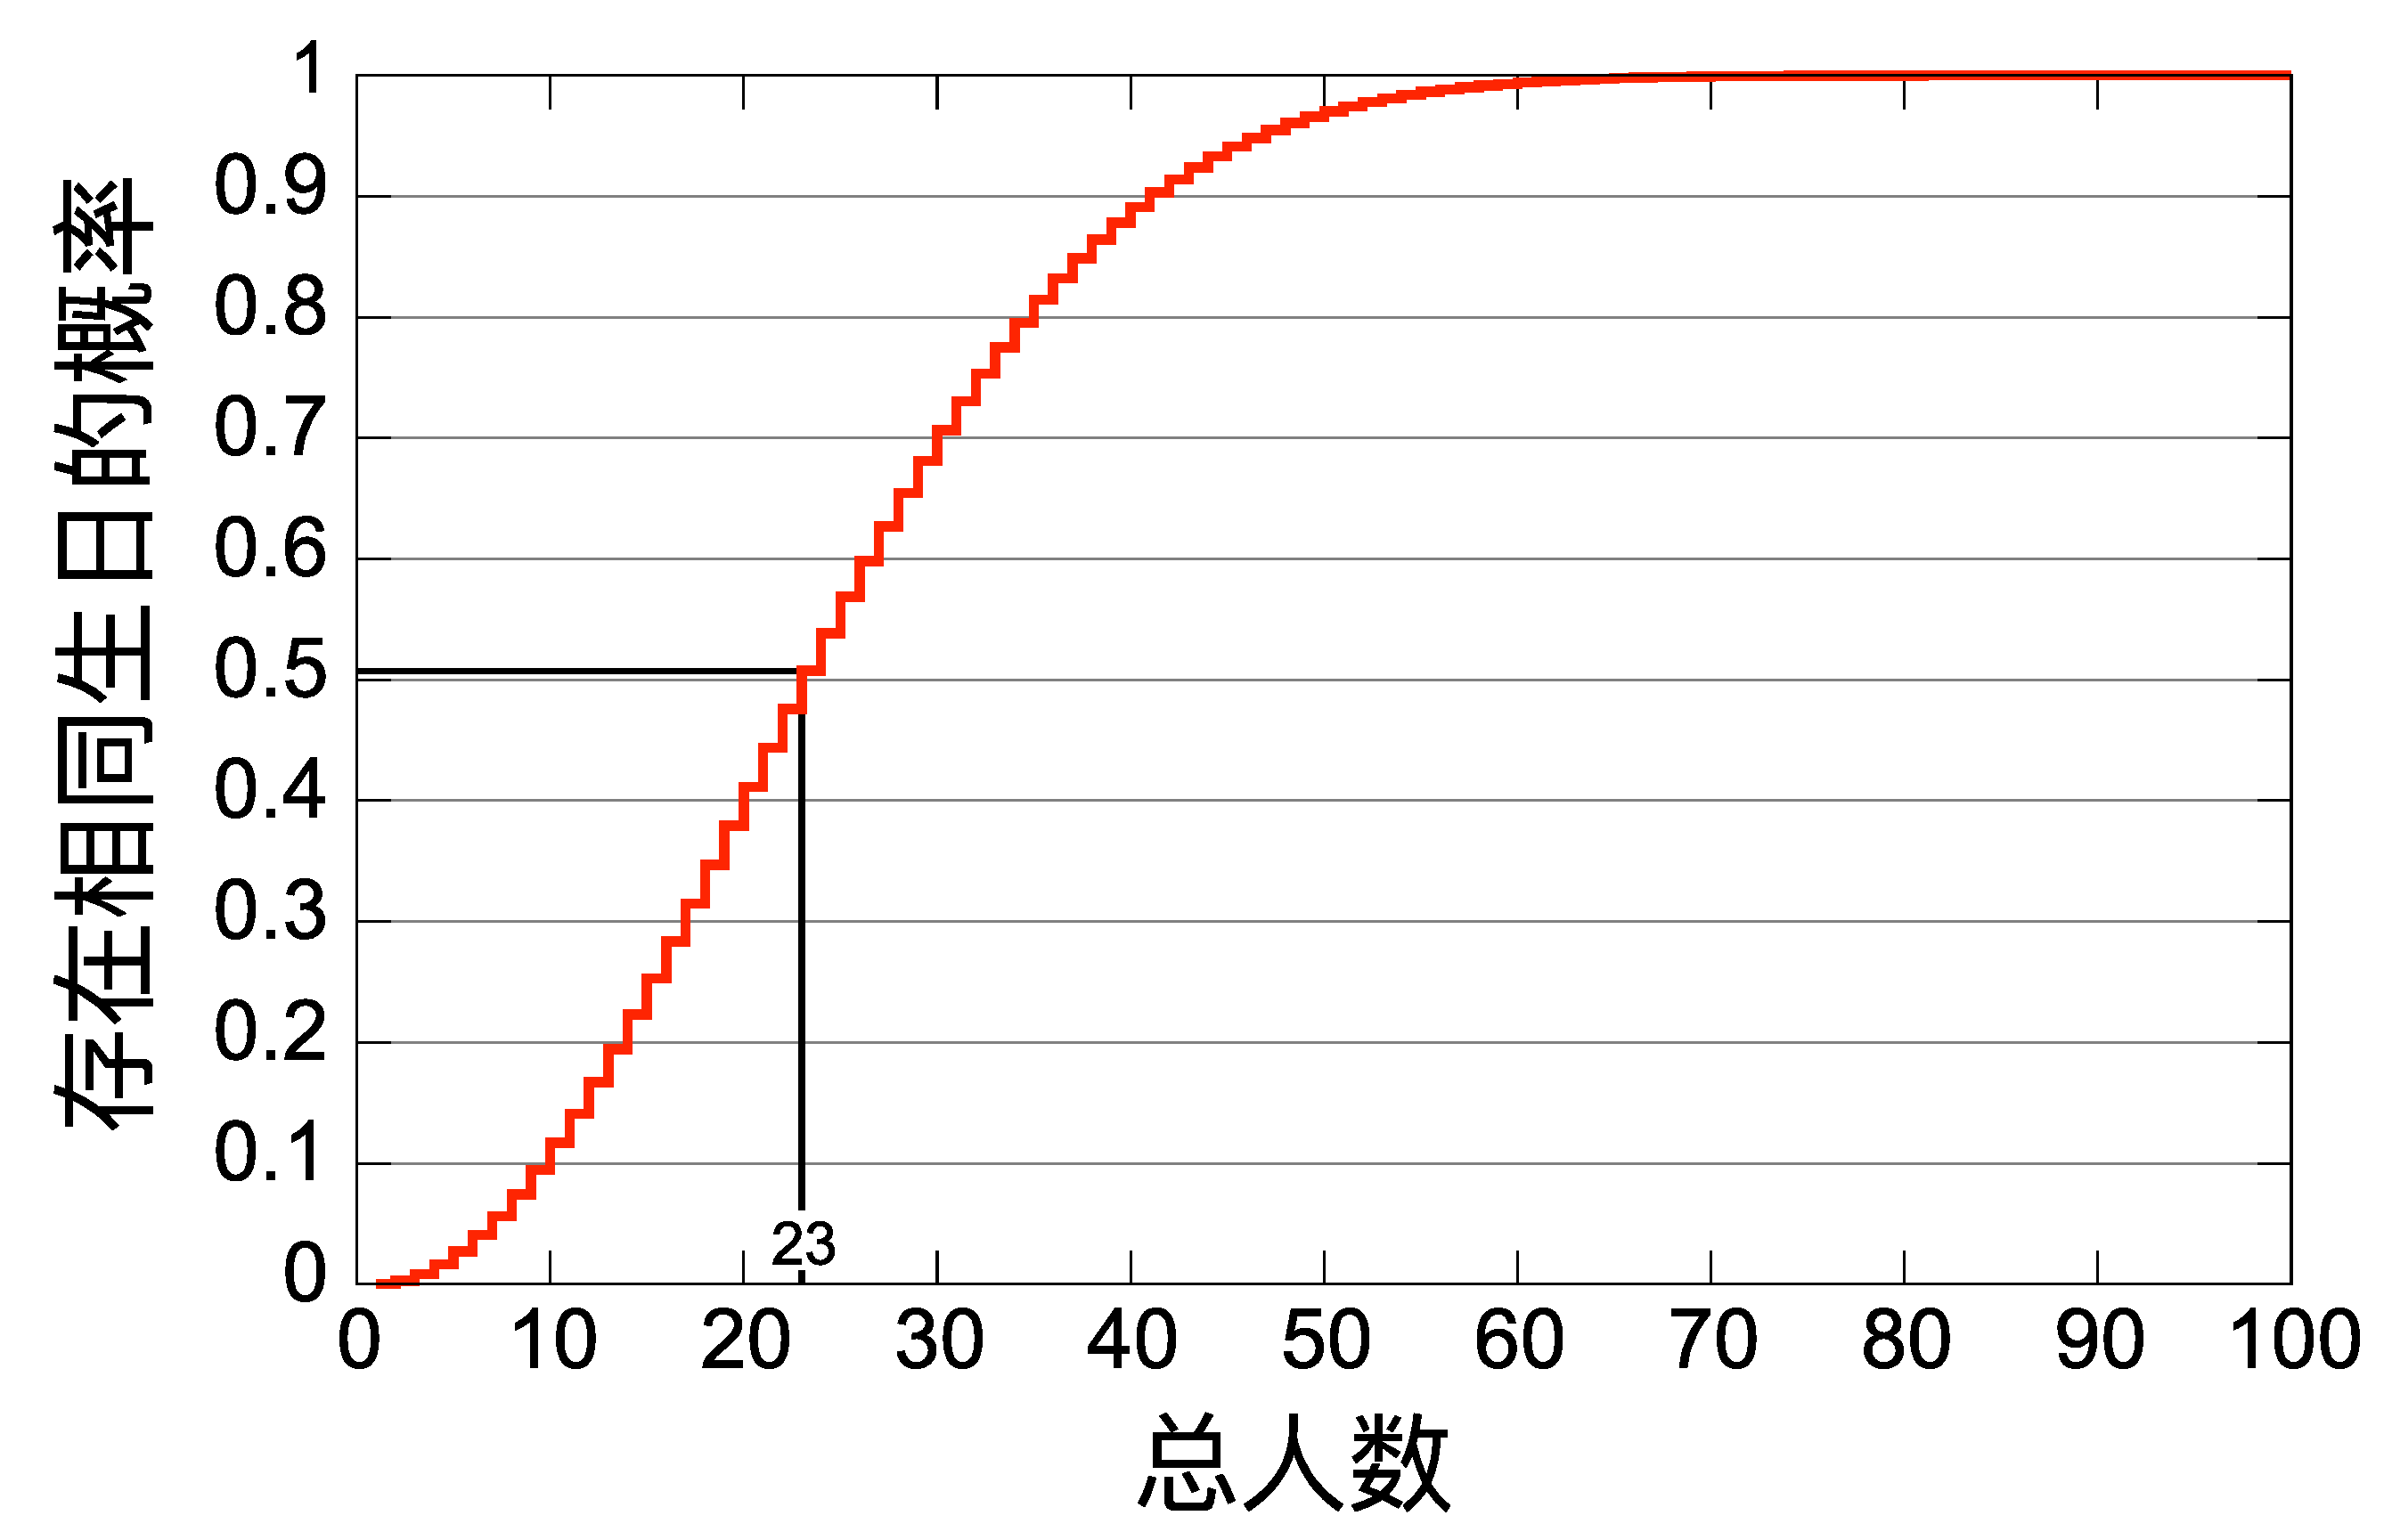
\includegraphics[width=.7\textwidth]{res/birthday_prob.pdf}
    \end{figure}

\end{frame}

\begin{frame}
    \frametitle{生日问题}

    \begin{problem}
        一般地,假设一年有 $n$ 天,班级中有 $k$ 个人,则班级中有两个人生日相同的概率 $p(n, k)$ 是多少?
    \end{problem}

    \[p(n, k) = 1 - (1 - \frac{1}{n}) \times \cdots \times (1 - \frac{k}{n})\]

    利用 $e^{-x} \approx 1 - x$,有

    \[p(n, k) \approx 1 - e^{-(1/n + 2/n + \dots + k/n)} = 1 - e^{-\frac{k(k - 1)}{2n}}\]

\end{frame}

\begin{frame}
    \frametitle{生日问题}

    要使 $p(n, k) = \frac{1}{2}$,大约需要多少人?

    \[\begin{split}
        1 - e^{-\frac{k(k - 1)}{2n}} = & \frac{1}{2} \\
        \frac{k(k - 1)}{2n} = & \ln 2 \\
        (k - \frac{1}{2})^2 = & 2n\ln 2 + \frac{1}{4} \\
        k = & \frac{1}{2} + \sqrt{2n\ln 2 + \frac{1}{4}} \\
        k \approx & \sqrt{2n\ln 2} \approx 1.2 \sqrt{n}
    \end{split}\]

    一般地,要使$p(n, k) = \varepsilon$,大约需要 $k \approx \sqrt{2n\ln \frac{1}{1 - \varepsilon}}$ 个人。

\end{frame}

\section{哈希碰撞}

\begin{frame}
    \frametitle{哈希函数}

    \begin{block}{哈希函数}
        一个哈希函数(如 MD5)将一个任意长度的字符串映射到固定大小的输出(如 128 bits)。
    \end{block}

    \begin{block}{示例}
        \begin{center}
            \fcolorbox{black}{gray!30}{\parbox{.9\linewidth}{你说的对,但是《原神》是由米哈游自主研发的一款全新开放世界冒险游戏。游戏发生在一个被称作「提瓦特」的幻想世界,在这里,被神选中的人将被授予「神之眼」,导引元素之力。你将扮演一位名为「旅行者」的神秘角色,在自由的旅行中邂逅性格各异、能力独特的同伴们,和他们一起击败强敌,找回失散的亲人。}}
        \end{center}
        \[\Downarrow MD5\]
        \begin{center}
            \fcolorbox{black}{gray!30}{\parbox{.55\linewidth}{D40525E634075A1058E930C0EF003E96}}
        \end{center}
    \end{block}

\end{frame}

\begin{frame}
    \frametitle{哈希函数}

    安全的哈希函数可以用于构造加密算法和数字签名算法

    \vline

    安全的哈希函数需要满足:

    \begin{enumerate}
        \item 对于随机的输入,输出是均匀随机的
        \item 给定输出$y$,很难找到$x$,使得$h(x)=y$
        \item 给定输入$x$,很难找到$x'$,使得$h(x)=h(x')$
        \item 很难找到 $x$ 和 $x'$,使得$h(x)=h(x')$(哈希碰撞)
    \end{enumerate}

\end{frame}

\begin{frame}
    \frametitle{哈希碰撞}
    
    \begin{block}{哈希碰撞}
        根据抽屉原理,无限个输入对应有限个输出,必然存在$x_1,x_2$,使得\[h(x_1)=h(x_2)\]
    \end{block}

    如果能快速找到哈希碰撞,将对哈希函数的安全性造成威胁

    \vline

    如何找到哈希碰撞?

    对输出长度为 $128$ bits 的哈希函数,枚举 $2^{128} + 1$ 个不同输入,根据鸽笼原理,必有一对哈希碰撞。

    是否有更好的方法?

\end{frame}

\begin{frame}
    \frametitle{生日攻击}

    \begin{block}{生日问题}
        假设一年有 $n$ 天,班级中有 $k$ 个人,则班级中有两个人生日相同的概率是多少?
    \end{block}

    \begin{block}{哈希碰撞}
        假设哈希函数有 $n$ 种可能的输出,随机选取 $k$ 个输入,则存在两个输入对应同一个输出的概率是多少?
    \end{block}

    均为 $p(n, k) = 1 - (1 - \frac{1}{n}) \times \cdots \times (1 - \frac{k}{n})$

    \vline

    当 $n = 2^{128}$ 时,要令 $p(n, k)\approx \frac{1}{2}$,只需尝试 $k\approx 1.2 \sqrt{n} \approx 2^{64}$ 次,远小于 $2^{128}$

\end{frame}

\begin{frame}
    \frametitle{对 MD5 的攻击}

    假设一台计算机 1 秒能进行 $10^9$ 次运算,需要

    \[\frac{2^{64}}{10^9} \ \text{s} \approx \frac{16\times 10^{18}}{10^9} \ \text{s} = 16 \times 10^9 \ \text{s} \approx 507 \ \text{year}\]

    \begin{columns}
        \column{0.7\textwidth}

        2005 年,王小云提出了一种对 MD5 的攻击,能够在 15 分钟到 1 小时内找到一组哈希碰撞。

        \vline

        \begin{itemize}
            \item 目前认为不安全的哈希算法(均被发现碰撞):MD5,SHA-0,SHA-1
            \item 目前认为仍然安全的哈希算法:SHA-2,SHA-3
        \end{itemize}

        \column{0.25\textwidth}

        \begin{figure}
            \centering
            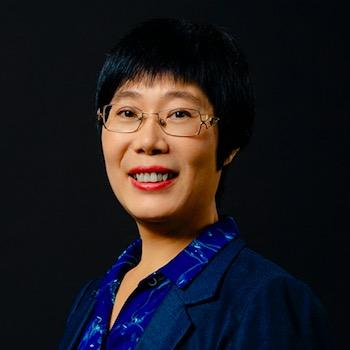
\includegraphics[width=\textwidth]{res/xiaoyunwang.jpg}
            \caption{王小云院士}
        \end{figure}
    \end{columns}

\end{frame}

\end{document}